
%%%
% Plantilla de Memoria
% Modificación de una plantilla de Latex de Nicolas Diaz para adaptarla 
% al castellano y a las necesidades de escribir informática y matemáticas.
%
% Editada por: Mario Román
%
% License:
% CC BY-NC-SA 3.0 (http://creativecommons.org/licenses/by-nc-sa/3.0/)
%%%

%%%%%%%%%%%%%%%%%%%%%%%%%%%%%%%%%%%%%%%%%
% Thin Sectioned Essay
% LaTeX Template
% Version 1.0 (3/8/13)
%
% This template has been downloaded from:
% http://www.LaTeXTemplates.com
%
% Original Author:
% Nicolas Diaz (nsdiaz@uc.cl) with extensive modifications by:
% Vel (vel@latextemplates.com)
%
% License:
% CC BY-NC-SA 3.0 (http://creativecommons.org/licenses/by-nc-sa/3.0/)
%
%%%%%%%%%%%%%%%%%%%%%%%%%%%%%%%%%%%%%%%%%

%----------------------------------------------------------------------------------------
%	PAQUETES Y CONFIGURACIÓN DEL DOCUMENTO
%----------------------------------------------------------------------------------------
%%% Configuración del papel.
% microtype: Tipografía.
% mathpazo: Usa la fuente Palatino.
\documentclass[a4paper, 11pt]{article}
\usepackage[protrusion=true,expansion=true]{microtype}
\usepackage{mathpazo}


% Indentación de párrafos para Palatino
\setlength{\parindent}{0pt}
  \parskip=8pt
\linespread{1.05} % Change line spacing here, Palatino benefits from a slight increase by default


%%% Castellano.
% noquoting: Permite uso de comillas no españolas.
% lcroman: Permite la enumeración con numerales romanos en minúscula.
% fontenc: Usa la fuente completa para que pueda copiarse correctamente del pdf.
\usepackage[spanish,es-noquoting,es-lcroman]{babel}
\usepackage[utf8]{inputenc}
\usepackage[T1]{fontenc}
\selectlanguage{spanish}


%%% Gráficos
\usepackage{graphicx} % Required for including pictures
\usepackage{wrapfig} % Allows in-line images
\usepackage[usenames,dvipsnames]{color} % Coloring code

%%% Matemáticas
\usepackage{amsmath}
%% comentarios multiples
\usepackage{verbatim}
\begin{comment}
	ejemplo
\end{comment}


%%% Bibliografía
\makeatletter
\renewcommand\@biblabel[1]{\textbf{#1.}} % Change the square brackets for each bibliography item from '[1]' to '1.'
\renewcommand{\@listI}{\itemsep=0pt} % Reduce the space between items in the itemize and enumerate environments and the bibliography
\usepackage{hyperref}
\hypersetup{
	colorlinks   = true,    % Colours links instead of ugly boxes
	urlcolor     = red,    % Colour for external hyperlinks
	linkcolor    = red,    % Colour of internal links
	citecolor    = blue      % Colour of citations
}

%%% CÓDIGO
\usepackage{listings}
\usepackage{courier}
\usepackage{xcolor}
\lstset{
	commentstyle=\itshape\color{purple!40!black},
	basicstyle=\footnotesize\ttfamily, % Standardschrift
	numbers=left,               % Ort der Zeilennummern
	numberstyle=\tiny,          % Stil der Zeilennummern
	%stepnumber=2,               % Abstand zwischen den Zeilennummern
	numbersep=5pt,              % Abstand der Nummern zum Text
	tabsize=2,                  % Groesse von Tabs
	extendedchars=true,         %
	breaklines=true,            % Zeilen werden Umgebrochen
	keywordstyle=\color{red}\bf,
	frame=b,         
	%       keywordstyle=[1],    % Stil der Keywords
	%        keywordstyle=[2]\textbf,    %
	%        keywordstyle=[3]\textbf,    %
	%        keywordstyle=[4]\textbf,   \sqrt{\sqrt{}} %
	stringstyle=\color{orange}\ttfamily, % Farbe der String
	showspaces=false,           % Leerzeichen anzeigen ?
	showtabs=false,             % Tabs anzeigen ?
	xleftmargin=17pt,
	framexleftmargin=17pt,
	framexrightmargin=5pt,
	framexbottommargin=4pt,
	%backgroundcolor=\color{lightgray},
	showstringspaces=false      % Leerzeichen in Strings anzeigen ?   
	literate=
	{á}{{\'a}}1 {é}{{\'e}}1 {í}{{\'i}}1 {ó}{{\'o}}1 {ú}{{\'u}}1
	{Á}{{\'A}}1 {É}{{\'E}}1 {Í}{{\'I}}1 {Ó}{{\'O}}1 {Ú}{{\'U}}1
	{à}{{\`a}}1 {è}{{\`e}}1 {ì}{{\`i}}1 {ò}{{\`o}}1 {ù}{{\`u}}1
	{À}{{\`A}}1 {È}{{\'E}}1 {Ì}{{\`I}}1 {Ò}{{\`O}}1 {Ù}{{\`U}}1
	{ä}{{\"a}}1 {ë}{{\"e}}1 {ï}{{\"i}}1 {ö}{{\"o}}1 {ü}{{\"u}}1
	{Ä}{{\"A}}1 {Ë}{{\"E}}1 {Ï}{{\"I}}1 {Ö}{{\"O}}1 {Ü}{{\"U}}1
	{â}{{\^a}}1 {ê}{{\^e}}1 {î}{{\^i}}1 {ô}{{\^o}}1 {û}{{\^u}}1
	{Â}{{\^A}}1 {Ê}{{\^E}}1 {Î}{{\^I}}1 {Ô}{{\^O}}1 {Û}{{\^U}}1
	{œ}{{\oe}}1 {Œ}{{\OE}}1 {æ}{{\ae}}1 {Æ}{{\AE}}1 {ß}{{\ss}}1
	{ű}{{\H{u}}}1 {Ű}{{\H{U}}}1 {ő}{{\H{o}}}1 {Ő}{{\H{O}}}1
	{ç}{{\c c}}1 {Ç}{{\c C}}1 {ø}{{\o}}1 {å}{{\r a}}1 {Å}{{\r A}}1
	{€}{{\euro}}1 {£}{{\pounds}}1 {«}{{\guillemotleft}}1
	{»}{{\guillemotright}}1 {ñ}{{\~n}}1 {Ñ}{{\~N}}1 {¿}{{?`}}1   
}

\usepackage{tikz}
%\DeclareCaptionFont{blue}{\color{blue}} 

%\captionsetup[lstlisting]{singlelinecheck=false, labelfont={blue}, textfont={blue}}
\usepackage{caption}
\DeclareCaptionFont{white}{\color{white}}
\DeclareCaptionFormat{listing}{\colorbox[cmyk]{0.43, 0.35, 0.35,0.01}{\parbox{\textwidth}{\hspace{15pt}#1#2#3}}}
\captionsetup[lstlisting]{format=listing,labelfont=white,textfont=white, singlelinecheck=false, margin=0pt, font={bf,footnotesize}}

%% cosas 

\usepackage[margin=1in]{geometry}

\usepackage{times}








%----------------------------------------------------------------------------------------
%	DOCUMENTO
%----------------------------------------------------------------------------------------

\begin{document}
	
	
	\begin{titlepage}
		\begin{center}

			
			{\Huge \textbf{INTELIGENCIA ARTIFICIAL \\Practica 1: Agentes reactivos.}\\
			Documentación del \\ comportamiento del agente.	}
			
			
		    \centering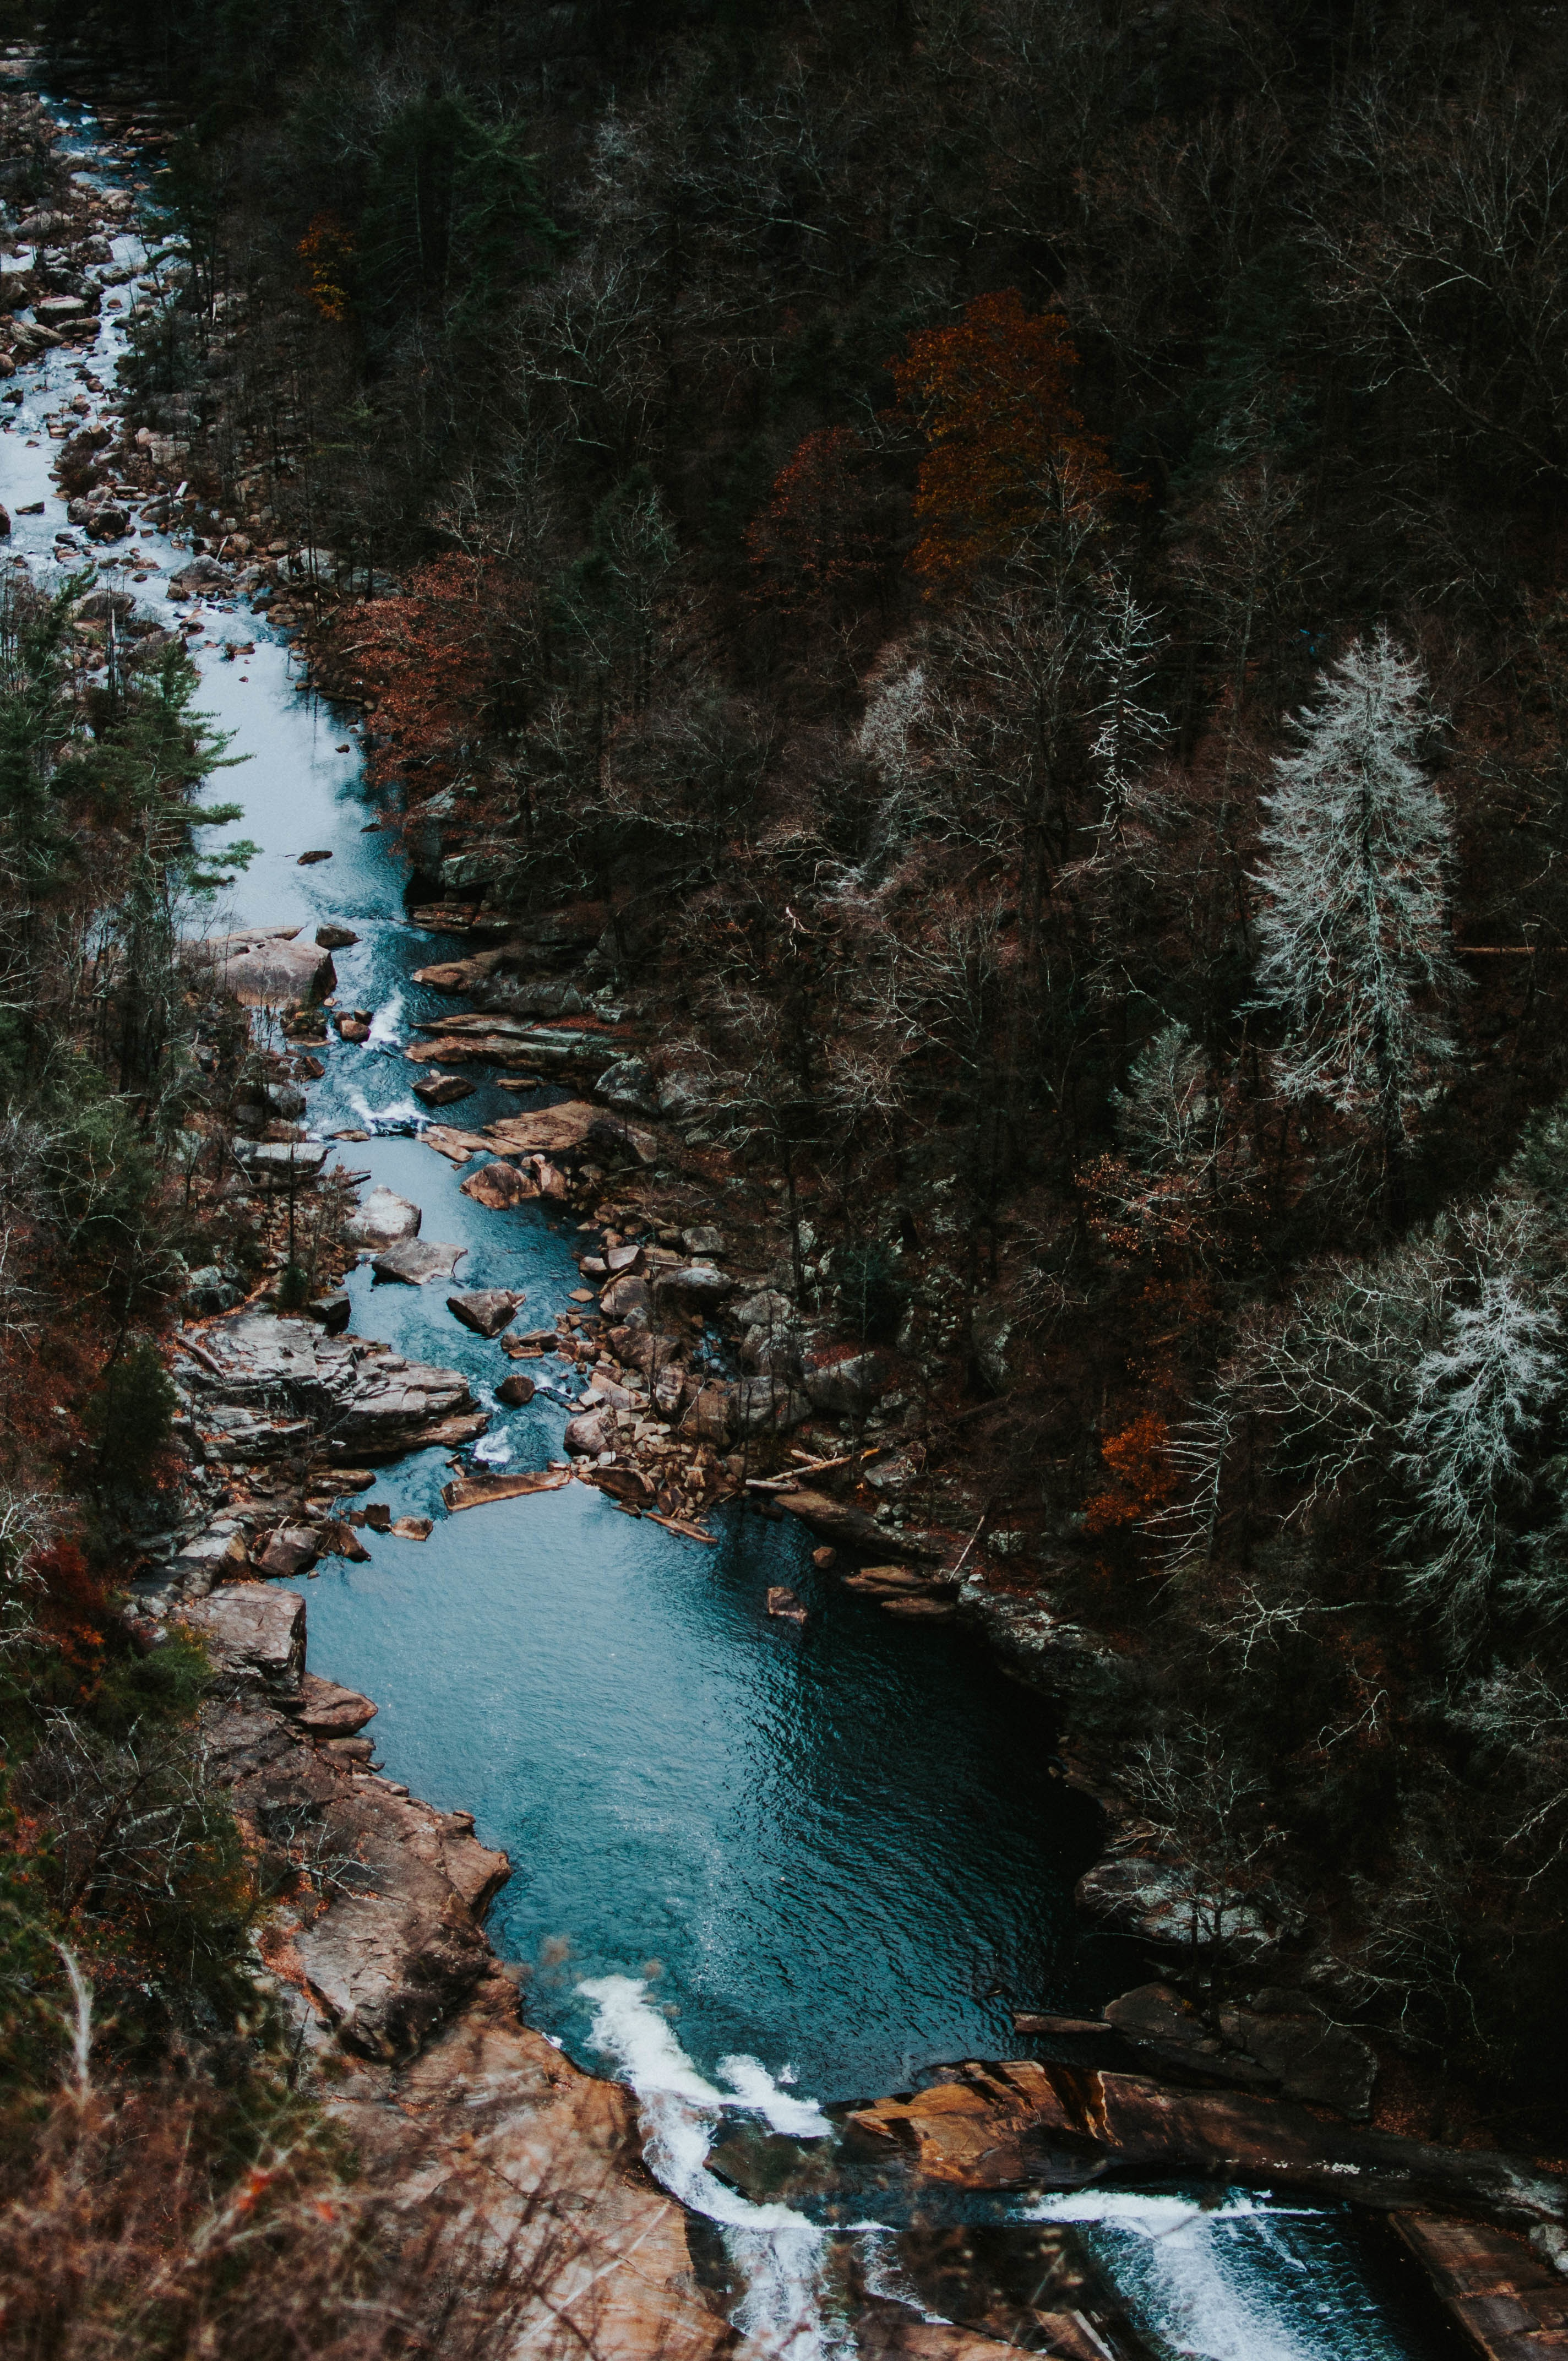
\includegraphics[width=0.71\textwidth]{cover.jpg}
		    
		    {\footnotesize Photo By: kazuend on unsplash.com } 
			
			
			\textbf{Francisco Navarro Morales - GRG121 }
			
			Segundo curso del Grado de Ingeniería Informática\\
			Universidad de Granada\\
			curso 2016-2017\\
			
		\end{center}
	\end{titlepage}


%\maketitle % Print the title section

%% Resumen (Descomentar para usarlo)
\renewcommand{\abstractname}{Resumen} % Uncomment to change the name of the abstract to something else
%\begin{abstract}
% Resumen aquí
%\end{abstract}

%% Palabras clave
%\hspace*{3,6mm}\textit{Keywords:} lorem , ipsum , dolor , sit amet , lectus % Keywords
%\vspace{30pt} % Some vertical space between the abstract and first section



%%% Inicio del documento

\pagebreak

\section{Movimiento.}
El agente ha utilizado tres métodos para elegir el próximo movimiento. El primero consiste en mantener una matriz `memoria' de enteros, inicializada a cero e ir sumando uno a cada casilla que el agente pise [fig. 2]. Así, las casillas con más valor son aquellas por las que se ha pasado más veces. El otro método es similar pero no suma uno a la casilla que pisa, sino que se le da el valor de un `contador' o reloj, que empieza a 0 y va aumentando en cada turno [fig. 1]. Así, no se controla cuantas veces se ha pasado por una casilla, sino que se controla cuáles son las últimas casillas por las que se ha pasado. La combinación consiste en utilizar el segundo método pero en lugar de asignar el valor del contador a la casilla, se le suma. De forma que a la hora de comparar casillas se tiene en cuenta cuál es la última que se ha pisado y, además, cuantas veces se ha pisado [fig. 3]. 

\begin{tikzpicture}
\foreach \x in {1,2,...,5,7,8,...,11,13,14,15,16,17}
\foreach \y in {1,...,5}
{
	\draw (\x,\y) +(-.5,-.5) rectangle ++(.5,.5);
}

\foreach \x in {1,2,5,7,8,10,11,13,14,17}
\foreach \y in {1,2,3,5}
	\draw (\x,\y) node{0};
	
	\draw (3,4) +(-.6,-.6) rectangle ++(.6,.6);
	\draw (9,4) +(-.6,-.6) rectangle ++(.6,.6);
	\draw (15,4) +(-.6,-.6) rectangle ++(.6,.6);
	\draw (3,1) node{1};
	\draw (4,1) node{0};
	\draw (3,2) node{2};
	\draw (4,2) node{0};
    \draw (3,3) node{3};
	\draw (4,3) node{0};
    \draw (3,4) node{14};
	\draw (4,4) node{13};
	\draw (3,5) node{9};
	\draw (4,5) node{0};
	\draw (1,4) node{6};
	\draw (2,4) node{7};
	\draw (5,4) node{12};
	
	\draw (3+6,1) node{1};
	\draw (4+6,1) node{0};
	\draw (3+6,2) node{1};
	\draw (4+6,2) node{0};
	\draw (3+6,3) node{1};
	\draw (4+6,3) node{0};
	\draw (3+6,4) node{4};
	\draw (4+6,4) node{2};
	\draw (3+6,5) node{1};
	\draw (4+6,5) node{0};
	\draw (1+6,4) node{1};
	\draw (2+6,4) node{2};
	\draw (5+6,4) node{1};
	
	\draw (3+12,1) node{1};
	\draw (4+12,1) node{0};
	\draw (3+12,2) node{2};
	\draw (4+12,2) node{0};
	\draw (3+12,3) node{3};
	\draw (4+12,3) node{0};
	\draw (3+12,4) node{36};
	\draw (4+12,4) node{24};
	\draw (3+12,5) node{9};
	\draw (4+12,5) node{0};
	\draw (1+12,4) node{6};
	\draw (2+12,4) node{12};
	\draw (5+12,4) node{12};
	\draw (3,6) node{Fig 1};
    \draw (3+6,6) node{Fig 2};
	\draw (3+12,6) node{Fig 3};
\end{tikzpicture}

Así, si nos fijamos en las figuras y, teniendo en cuenta que a la hora de decidir qué dirección tomar solo se comparan los valores de enfrente, la derecha y la izquierda de dónde se encuentra el agente, y se elige el menor, y suponiendo que el agente mira hacia arriba en la casilla remarcada: en el caso de la izquierda el agente giraría a la izquierda; en el del centro, avanzaría; y en el de la derecha (el que he escogido) avanzaría.

Hay que tener en cuenta que el agente antes de pensar si quiera en girar a la derecha, la izquierda o avanzar, comprueba si dicha acción es posible (si no hay algún obstáculo que se lo impida). Así, en el ejemplo que he puesto, si en la casilla de arriba de dónde se encuentra el agente hubiera un obstáculo, en la segunda opción cogería cualquiera de las dos, izquierda o derecha, aleatoriamente; o bien, una establecida por defecto; mientras que en el caso de la derecha 	se giraría a la izquierda porque es por la que se pasó hace más tiempo de las dos. 

Aunque en un principio me pareció que el método que combinaba los otros dos era mejor, pero tras hacer pruebas vi que el método que solo comprueba cual se pisó menos recientemente da mejores resultados y decidí utilizar ese.

También es interesante señalar el uso de una función que establece casillas que no me interesa pisar, de forma que les asigna el valor actual de contador de tiempo más diez, de forma que durante los próximos turnos sea la última opción a elegir. Un ejemplo del uso de esta función es cuando el agente encuentra un lobo y no tiene ningún hueso que darle, entonces le asigna dicho valor a la casilla del lobo y así se obliga a sí mismo a girar y "huir" del lobo.

Además he introducido un factor `aleatorio' que obliga al agente a girar a la casilla mejor (izquierda o derecha) según el criterio establecido aunque la casilla del frente tuviera más prioridad y los resultados han sido buenos ya que, por ejemplo, cuando el agente (por la disposición de los obstáculos) realiza una trayectoria rectangular cerrada, tiende a repetir dicha trayectoria interiorizando en el rectángulo (haciéndolo cada vez más pequeño hasta haberlo pisado entero) y esto es bastante absurdo porque en cada vuelta al rectángulo solo va rellenando una casilla del borde cuando su visión le permitiría rellenar más. Al introducir el giro aleatorio se impide que de demasiadas vueltas a estos rectángulos (entre otras cosas). He escogido que se gire obligatoriamente cada veintitrés pasos tras probar a darle varios valores y ver que los mejores resultados se generaban con 42 y 23 pasos (con 23 eran un poco mejores así que elegí ese número).

\section{Objetos}
	Durante las sesiones de prácticas he `descubierto' que los huesos se pueden dar a los lobos para hacerlos desaparecer durante un par de turnos con la acción actGIVE, el bikini sirve para poder pisar las casillas de agua, las zapatillas para las casillas de bosque y la llave para abrir puertas (también con actGIVE). He tenido en cuenta que no se puede cambiar las zapatillas por el bikini para pasar de bosque a agua, o al revés, porque en el momento en que el agente se quita el objeto que lleva y le permite pisar la casilla en la que está, muere. 
	En un principio programé que cuando viera un objeto que ya tenía se lo equipara y lo tirara para coger el nuevo pero esto provocaba que hubiera pocos objetos en el mapa, por eso lo cambié a utilizar la función NoPisar sobre la casilla con el objeto para evitarlo. También hubiera sido interesante poder dejar el objeto en el suelo a un lado y luego coger el nuevo, pero por alguna razón me ha sido imposible hacer que el agente deje los objetos en el suelo (he probado todas las circunstancias que se me han ocurrido con todos los objetos y no los suelta), por lo que he concluido que era imposible (quizá por algún fallo en el programa Belkan o simplemente porque yo sería incapaz de encontrar las circunstancias requeridas a tiempo) y me he limitado a esquivar el objeto que ya tengo.
	
	Para `equipar' un objeto necesario para pisar un determinado terreno, abrir una puerta o eliminar a un lobo, lo que hace el agente es ver si tiene el objeto (para lo que mantiene un vector de booleanos con los objetos que posee y los que no) y, si lo tiene, comprueba si lo lleva encima, si no, comprueba si tiene algún otro objeto para guardarlo (actPUSH) y si no lleva ninguno coge algún objeto de la mochila (actPOP).

\section{Mapa}
He programado que todo lo que el agente ve se introduzca en el mapa resultado y además, he establecido una matriz auxiliar para ir guardando lo que ve cuando aún no está situado e introducirlo cuando se sitúa. También he introducido una matriz de memoria auxiliar para utilizar el método de movimiento cuando aún no se está situado.
Para situarse antes, he programado un módulo que hace que, si se ve una casilla de GPS frente al agente, se le obligue a avanzar aunque la mejor opción fuera girar y, si en la memoria se ha guardado una de estas casillas a izquierda o derecha del agente y las casillas que hay entre el agente y la casilla GPS se puden pisar, entonces gira en dicha dirección.

\section{Puertas}
Por último para asegurarme de que se abren las puertas, si el agente lleva una llave y tiene una puerta a la derecha o izquierda, gira obligatoriamente para mirar hacia ella, entonces la abre y pasa. El problema es que esto hace que una vez dentro vuelva a girar para abrirla y salir y no entra en la sala (e incluso se queda atascado). Por ello he creado una variable entera `abierta' que se pone a 5 cuando se abre la puerta y se va restando en una unidad cada turno desde entonces de forma que no se intente abrir la puerta otra vez si la variable es mayor que cero. 
\end{document}